\documentclass[french]{article}
\usepackage[utf8]{inputenc}
\usepackage[T1]{fontenc}
\usepackage{amsmath}
\usepackage{amsthm}
%\usepackage[amsmath]{ntheorem}
%\usepackage{ntheorem}
\usepackage{lmodern}
%\usepackage{kpfonts}

\usepackage{babel}

\newtheorem{definition}{Définition}
\newtheorem{theoreme}{Théorème}
\newtheorem{preuve}{Preuve}
\newtheorem{proposition}{Proposition}
\newtheorem{exemple}{Exemple}

\usepackage{graphicx}

\usepackage[np]{numprint}

\newcommand{\N}{\mathbb{N}}
\newcommand{\R}{\mathbb{R}}
\newcommand{\Z}{\mathbb{Z}}

\usepackage{multicol}

%\begin{filecontents}{\jobname.bib}
%  @book{Ramis-Deschamps-Odoux,
%    Author = {Edmond Ramis and Claude Deschamps and Jacques Odoux},
%    Origyear = {1974},
%    Publisher = {Masson},
%    Title = {Cours de mathématiques : 1. algèbre},
%  Year = {2001}}
%\end{filecontents}
%\usepackage{natbib}
%\bibliographystyle{apalike}

\title{Cryptographie et enjeux de société}
\author[jumelvin@jbs-ndc93.com]{Vincent-Xavier Jumel}
\date{12 février 2016}

\begin{document}
\section{Généralités}

  \maketitle

  Crypter = mettre dans une crypte

  \begin{itemize}
    \item Chiffre de César
    \item Chiffre de Vigenère
    \item Enigma
    \item RSA
    \item Courbes elliptiques
    \item Else …
  \end{itemize}

    
\includegraphics[width=0.8\linewidth]{Scytale.jpeg}

  \begin{multicols}{2}
      \begin{itemize}
        \item décalage de caractère
        \item constant
        \item facile à chiffrer
        \item facile à déchiffrer
      \end{itemize}
      \begin{itemize}
        \item A $\rightarrow$ D
        \item D $\rightarrow$ A
      \end{itemize}
      CESAR $\rightarrow$ GIWEV
  \end{multicols}

    \begin{itemize}
      \item Chiffre polyalphabétique ;
      \item Difficile à mettre en œuvre manuellement
      \item Fondamentalement peu résistant à l'analyse statistique
    \end{itemize}
    \scriptsize
    \begin{verbatim}
Texte en clair :   j'adore ecouter la radio toute la journee
Clé répétée    :   M USIQU EMUSIQU EM USIQU EMUSI QU EMUSIQU
                   ^ ^^^
                   | ||Colonne O, ligne I : on obtient la lettre W.
                   | |Colonne D, ligne S : on obtient la lettre V.
                   | Colonne A, ligne U : on obtient la lettre U.
                   Colonne J, ligne M : on obtient la lettre V.
    \end{verbatim}
  \normalsize

  \begin{multicols}{2}
    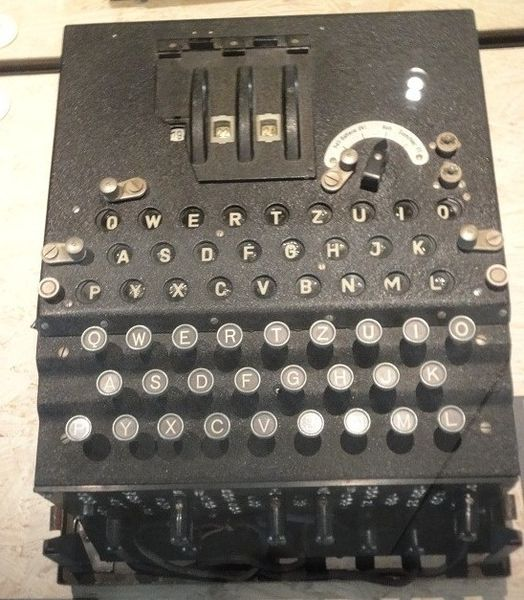
\includegraphics[width=0.45\linewidth]{524px-Enigma_1940.JPG}
    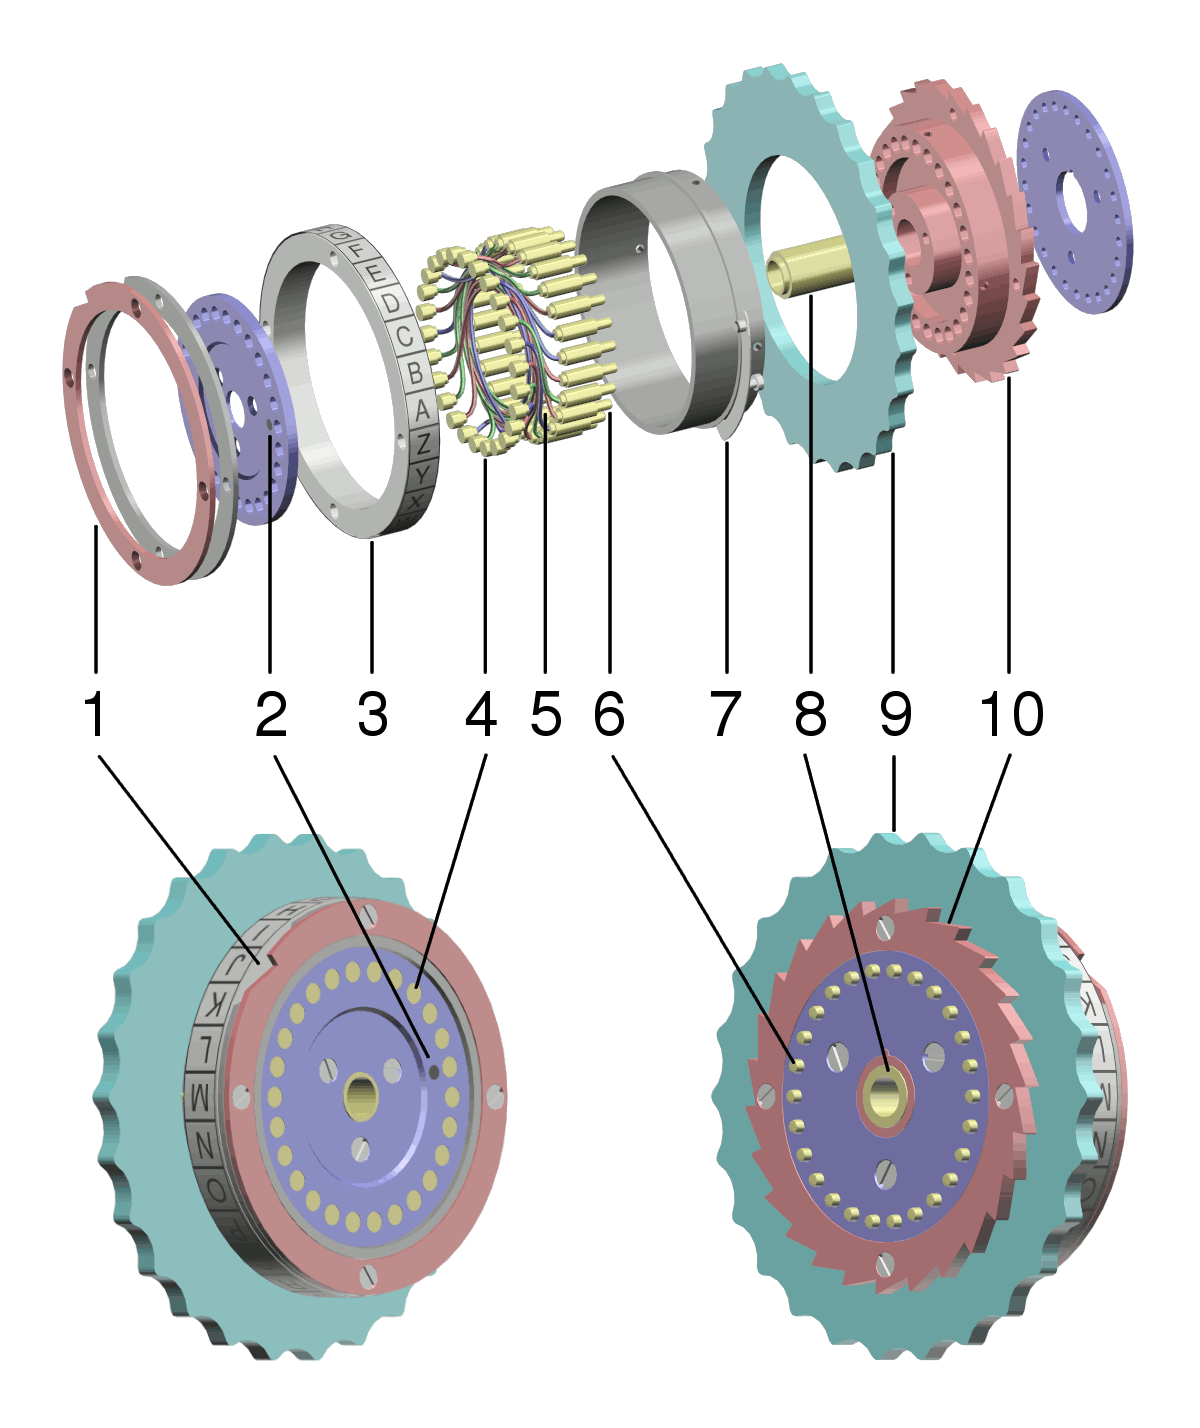
\includegraphics[width=0.45\linewidth]{Enigma_rotor_exploded_view.png}
  \end{multicols}
  \begin{multicols}{2}
      \begin{itemize}
        \item Le codage est un produit de permutations (des bijections)
        \item Un rotation du rotor est une permutation circulaire
        \item $\np{1.59}\times 10^{20}$ combinaisons (mais des produits
          de permutations)
      \end{itemize}
      \begin{verbatim}
- 186 - DOQ VHZ -

PBNXA SMDAX NOOYH RCZGV
VZCBI GIBGW HMXKR RVQCF
JCZPT UNSWA DDSTI GQQCS
AGPKR XXLOM GFXAP HHMRF
SDKYT MYPMV ROHAS QYRWF
WVAVG CCUDB IBXXD YZSAC
JSYOT MWUCN WOMHH JPYWD
CCLUP GSWCL MBCZS SYXPG
MGMQX AUFUL NOZEQ ENHEI
ZZAKL C
\end{verbatim}
  \end{multicols}

  \begin{multicols}{2}
      \begin{itemize}
        \item lettre $\leftrightarrow$ chiffre
        \item plusieurs codes : ASCII, UTF-8
      \end{itemize}
      \begin{itemize}
        \item A $\rightarrow$ 65
        \item a $\rightarrow$ 97
        \item é $\rightarrow$ 195 ou 233
      \end{itemize}
      CESAR $\rightarrow$ 067069083065082
  \end{multicols}

  \begin{itemize}
    \item langue complexe
    \item parlée par très peu de personnes
    \item un des rares code non cassé avec RSA
  \end{itemize}

    \begin{itemize}
      \item chiffrement asymétrique
      \item clef publique
      \item clef privée
      \item résistance à l'analyse statistique
    \end{itemize}

    \scriptsize
    \begin{verbatim}
      hQIMAzJEJPrLXcHlARAAutxmrtyxCqbzfRQStvTfpLAoo2hnTLO3Z6J21swH3fPR
      xzG9Il2jiigKtevPsDfBHo7dNzJgVLHfh7WbiV5NgVBawKS/NfKErLW+Ovy4QwR2
      nfaLguhOseZGFdsF4EYrJuW9Z6NcSXR1BCVvfNWpToLuZuKePKn5k+/H/rIUTxpv
      Cftk28du/CNM5qZMf43T0kbmoKiKJYhc0/Qud2+InftmDHyJV8lQWUX5FkMP9Mmo
      09w5Bk7qfClDMin7dG6SxXfzGGc6MiZrIr0NDFABqupp7x21KzeAJ2BrJ616whWr
      qrMPlRSxXf1yyGHCLtw50zv0J24tK3EPMV56sJTzklAR0NG+OmjHSLowkBywDzBC
      pxjklos4J3NU3Kcm9nt35n9Z3ABcnTcuPreu4bHcbPcvLc5kfsNWlAnlHb9RN2te
      OxJxOQNPLfIkILE3evCz6Vp00r9w80DfrVD8Yn9X3eGqxaF44Acp7tHc1xk1D4Kd
      NgBCvTi4F6Bk7YPDtb0oUZUjhINZnCfP2kyykun7XDmNFKUSRZxGFwK43a/tW/sg
      42OatKBgeywwqmIyu2pZRK8t2+IwDjJVK4828mDA3rj/3k0Hyuyhk8l2wCp9cJGf
      7CIhw2waAZLMKXW/L54o3NXxYrsnGd/fI63TbiMM+odEwJE5AIOFDWoLtpwTfEXS
      QAHDsj8u0mlT0+lxoIG/Icj6aDDakn1kZH6GwlIvis4sEOba9CCivaSzgNJiqDSL
      kt/m9iz7TXF/pW3GXRwiC3M=
      =YxRF
    \end{verbatim}
    \normalsize

\section{Le chiffrement asymétrique}

  \begin{multicols}{2}
      \begin{itemize}
        \item Alice veut parler à Bob
        \item Choix d'une clef secrète
        \item La clef sert à chiffrer et déchiffrer
      \end{itemize}
      \begin{itemize}
        \item facile à mettre en œuvre
        \item clef faible
        \item nécessité de renouvellement de la clef via un canal
          sécurisé
      \end{itemize}
  \end{multicols}

  \begin{multicols}{2}
      \begin{itemize}
        \item Alice veut parler à Bob
        \item Bob communique publiquement à Alice sa clef publique
        \item La clef sert uniquement à chiffrer
        \item Bob déchiffre le message avec sa clef privée
      \end{itemize}
      \begin{itemize}
        \item mise en œuvre plus complexe
        \item clef forte, mais double
        \item nécessité de s'assurer de l'identité du destinataire
      \end{itemize}
  \end{multicols}

  \begin{multicols}{2}
      \begin{itemize}
        \item Alice veut s'assurer que Bob reçoit un message qui :
          \begin{itemize}
            \item provient bien d'Alice
            \item n'a pas été altéré
          \end{itemize}
        \item Alice communique publiquement à Bob sa clef publique
        \item La clef signe le message avec sa clef privée
        \item Bob authentifie le message avec la clef publique d'Alice
      \end{itemize}
      \begin{itemize}
        \item mise en œuvre plus complexe
        \item clef forte, mais double
        \item nécessité de s'assurer de l'identité de l'expéditeur au
          préalable
      \end{itemize}
  \end{multicols}

\section{Principe mathématique}
  \begin{multicols}{2}
      \begin{itemize}
        \item Fonction «facile» à calculer
        \item mais difficile à «inverser»
      \end{itemize}
    \columnbreak
      \begin{itemize}
        \item un secret supplémentaire qui permet de retrouver le point
          de départ
        \item à ne pas confondre avec une «porte dérobée»
      \end{itemize}
  \end{multicols}

\section{Pratique du chiffrement et enjeux de sociétés}

  \begin{itemize}
    \item Protection des correspondances
    \item Paiement sécurisé sur un réseau non sécurisé
    \item Applications militaires
  \end{itemize}

  \begin{itemize}
    \item Avec de la surveillance : pas de liberté d'expression
    \item Sans garantie d'intégrité : pas de liberté d'expression
  \end{itemize}

  \begin{itemize}
    \item Fixer un prix de prestation dans un contexte concurrentiel
  \end{itemize}

  \begin{itemize}
    \item Espionnage industriel
    \item Espionnage commercial
    \item Liberté d'expression dans certains pays
  \end{itemize}

\section{Notions générales d'arithmétique}
  chiffrements}
  \begin{multicols}{2}
      \begin{itemize}
        \item ASCII
        \item Entiers / binaires
      \end{itemize}
    \columnbreak
      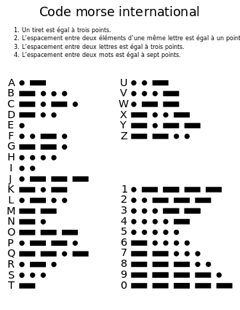
\includegraphics[width=0.45\linewidth]{330px-International_Morse_Code-fr.png}

      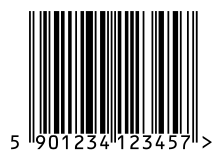
\includegraphics[width=0.45\linewidth]{File-EAN-13-5901234123457.png}
      
\includegraphics[width=0.45\linewidth]{Qr-4.png}
  \end{multicols}

  \begin{itemize}
    \item Nombres premiers
    \item Division euclidienne
    \item irréversibilité des opérations
  \end{itemize}

  \begin{definition}[Divisibilité]
    On dit que $a$ divise $b$ si et seulement s'il existe un nombre $c$
    tel que $b=ac$. On note $a\mid b$ si $a$ divise $b$ et $a \nmid
    b$ sinon.
  \end{definition}
  \begin{proposition}
    La relation $\mid$ est une relation d'ordre partiel
  \end{proposition}

  \begin{proposition}[Division euclidienne]
    Soient $a$ et $b$ deux nombres relatifs, $b\neq 0$, ($(a,b)\in
    \Z\times\Z^*$) ; il existe un entier relatif et un entier naturel
    tels que $a=bq+r$.

    Si on impose que $0\leq r<b$, alors $q$ et $r$ sont uniques.
  \end{proposition}

  \begin{proof}
    Soient $a\in\Z$ et $b\in\Z^*$. Supposons qu'il existe deux couples
    $(q,r)$ et $(q',r')$ tels que $0 \leq r<b$ et $0\leq r'<b$ et $a =
    bq + r = bq' + r'$.  \[ \implies b(q - q') = r' - r \] or $r' - r
    \nmid b$, donc $r' - r = 0$ et $q -q'=0$, car $b\neq 0$.
  \end{proof}

  \begin{definition}[classes de congruence]
    On note $n\Z = \left\lbrace kn, n\in\Z \right\rbrace$ ; on dit que
    $x$ est congru à $y$ modulo $n$ et on note $x\equiv y \mod n \iff
    x-y \in n\Z$.

    On note $\overline{x}$ les éléments congrus à $x$ modulo $n$ ;
    l'ensemble des classes de congruences $\left\lbrace \bar0, \bar1,
    \bar2, …, \overline{n-1} \right\rbrace = \Z/n\Z$.
  \end{definition}

\section{Généralités d'algèbre générale}

  \begin{definition}
    On appelle \emph{groupe} tout ensemble muni d'une loi
    \begin{itemize}
      \item possédant un élément neutre (1 ou 0) ;
      \item où toute combinaison d'élément appartient encore à
        l'ensemble ;
      \item où tout élément possède un inverse
    \end{itemize}
    S'il est commutatif, on dit aussi qu'il est abélien.
  \end{definition}
  \begin{proposition}
    $\Z/n\Z$ est un groupe pour l'addition.
  \end{proposition}
  \begin{definition}[anneau]
    Un anneau est un groupe $G$ abélien pour une loi (notée +) et
    possède une loi (notée $\times$) distributive sur $+$.
  \end{definition}
  \begin{proposition}
    $(\Z,+,\times)$ est un anneau.
  \end{proposition}
  \begin{definition}[intègre]
    On dit qu'un anneau est intègre $\iff ab = 0 \implies a = 0$ ou $b =
    0$.
  \end{definition}
  \begin{definition}[corps]
    Un corps est un anneau où tous les éléments non nuls sont
    inversibles.
  \end{definition}

  \begin{definition}
    $a \equiv b [n] \iff a = q\times n + b,\ q\in\Z $
  \end{definition}
  \begin{proposition}
    $a \equiv b [n] \iff a - b \equiv 0 [n] $
  \end{proposition}
  \begin{proposition}
    La proposition précédente se lit également : «$b$ est le reste de
    la division euclidienne de $a$ par $n$.»
  \end{proposition}

  \begin{proposition}
    $(\Z/nZ,+,\times)$ est un corps si et seulement si $n$ est premier.
  \end{proposition}
  \begin{proof}
    \begin{itemize}
      \item $\bar{k}$ est inversible dans $\Z/n\Z \iff k\wedge n = 1$.
        Si $n$ est premier, $\forall k < n, k\wedge n = 1$, d'où
        $\bar{k}$ est inversible.
      \item Si $\Z/n\Z$ est un corps, il possède $n-1$ éléments
        inversibles. $\implies n$ est premier avec tous les éléments de
        1 à $n-1$. N'ayant pas d'autres diviseurs que 1 ou lui-même, il
        est premier.
    \end{itemize}
  \end{proof}

  \begin{proposition}
    Soient $a_1, a_2, …, a_n$ des entiers non nuls ; il existe un unique
    entier $d$ tel que $a_1\Z + a_2\Z + \cdots + a_n\Z = d\Z$
    \begin{proof}
      \begin{itemize}
        \item Les sous groupes additifs de $\Z$ sont de le forme $a\Z$
        \item Si $G_1$ et $G_2$ sont des sous groupes d'un groupe
          «additif», alors $G_1 + G_2$ est un sous groupe.
      \end{itemize}
    \end{proof}
  \end{proposition}

  \begin{definition}[bijection]
    Une application $f:E\to F$ qui fait correspondre à tous les éléments
    de $E$ un unique élément de $F$ s'appelle une bijection.
  \end{definition}
  \begin{definition}[morphisme]
    Une application d'une structure algèbrique vers la même structure
    algébrique qui conserve la compatibilité des opérations est un
    morphisme.

    On dit isomorphisme quand les ensembles sont les mêmes.
  \end{definition}
  \begin{exemple}
    $f:\Z\to\R,\ n\mapsto a^n$ est un morphisme de groupe.
  \end{exemple}
  \begin{definition}[noyau]
    $\lbrace x\in G \mid f(x) = 0_G \rbrace$ est un sous groupe du
    groupe $(G,+)$, noté $\ker f$.
  \end{definition}
  \begin{proposition}
    $f$ est injective $\iff \ker f = {0_G}$
  \end{proposition}
  \begin{definition}[cardinal]
    Le nombre d'éléments d'un ensemble s'appelle son cardinal et est
    noté $\mathop{Card} E$.

    On dit qu'il est fini si $\mathop{Card} E < +\infty$.
  \end{definition}
  \begin{proposition}[ensemble produit]
    $E\times F$ est l'ensemble des couples d'éléments de la forme $(x\in
    E; y\in F)$.

    Cet ensemble est de cardinal $\mathop{Card} E \times \mathop{Card}
    F$.
  \end{proposition}
  \begin{proposition}
    Soit $f:E\to F$, deux ensembles finis. Il y'a équivalence entre :
    \begin{itemize}
      \item $f$ injective
      \item $f$ bijective
    \end{itemize}
  \end{proposition}
  \begin{definition}[ordre d'un élément]
    C'est l'entier naturel telque $a^n = 1$ dans un groupe noté
    multiplicativement
  \end{definition}
  \begin{definition}[groupe cyclique]
    C'est un groupe ou tout élément peut s'écrire $a^n$ (notation
    multiplicative).
  \end{definition}

\section{Arithmétique plus avancée}

  \begin{definition}
    \begin{itemize}
      \item Le nombre $d$ de la proposition précédente est le
        \emph{pgcd}. On note $a_1 \wedge a_2 \wedge … \wedge a_n = d$.
      \item Si $d=1$, on dit que les nombres sont premiers dans leur
        ensemble.
    \end{itemize}
  \end{definition}
  \begin{proof}
    $d=a\wedge b \neq 0 \implies d\mid a$ et $d\mid b$ et c'est bien le
    plus grand.
  \end{proof}

  \begin{theorem}[Bezout]
    $a\wedge b = 1 \iff \exists (u,v)\in\Z^2,\ au+bv = 1$
  \end{theorem}
  \begin{proof}
    \begin{itemize}
      \item $a\wedge b = 1 \implies a\Z + b\Z = \Z$
      \item Soient $(u,v)\in\Z^2,\ au+bv = 1 \implies 1\in a\Z + b\Z
        \implies \Z\subset a\Z + b\Z$, d'où l'égalité d'ensemble et donc
        l'égalité.
    \end{itemize}
  \end{proof}
  \begin{theorem}[Gauss]
    Si $a\mid(bc)$ et $a\wedge b = 1$, alors $a\mid c$.
  \end{theorem}
  \begin{proof}
    Bezout $\implies au + bv = 1 \implies acu + bcv = c$.

    Or $a\mid acu$ et $a\mid bcv$ donc $a\mid c$.
  \end{proof}


  \begin{definition}[Nombres premiers]
    Un nombre premier est un nombre qui n'est divisible que par 1 et
    lui-même.
  \end{definition}
  \begin{theorem}[Infinité des nombres premiers]
    Il y'a une infinitié de nombres premiers
  \end{theorem}
  \begin{proof}
    Supposons que l'ensemble des nombres premiers soit fini. Prenons le
    produit de tous les nombres premiers augmenté de 1. Ce nombre n'est
    divisible par aucun des nombres premiers précédents. Ce nombre est
    donc plus grand, ce qui contredit l'hypothèse initiale
  \end{proof}

  \begin{theorem}[Décomposition]
    Soit $n$ un nombre entier. Il existe une unique décomposition, à
    l'ordre près, de $n$ en produit de nombres premiers $p_1,\dots,p_r$
    et $n = p_1^{\nu_1}\times\cdots\times p_k^{\nu_k}$.
  \end{theorem}
  \begin{proof}
    \begin{itemize}
      \item Tout entier $n\geq 2$ admet un facteur premier $p$ tel que
        $n=pn_1$, $n_1<n$
      \item si $n_1$ n'est pas premier, alors il est composé. En un
        nombre fini d'étape, on aboutit à la décomposition
      \item S'il existe deux décompositions, $p_1^{\nu_1}\times
        \cdots\times p_k^{\nu_k}$ et $p_1^{\nu'_1}\times \cdots\times
        p_k^{\nu'_k}$, alors $p_1^{\nu_1} \mid p_1^{\nu'_1}$, car
        étranger à tous les autres, d'où $\nu_1 \leq \nu'_1$ et par
        symétrie $\nu_1 \geq \nu'_1$ et donc l'égalité.
    \end{itemize}
  \end{proof}


  \begin{theorem}[des chinois]
    $\Z/m\Z\times \Z/n\Z$ et $\Z/mn\Z$ sont isomorphes.
  \end{theorem}
  \begin{proof}
    On considère l'application $f:\Z\to\Z/m\Z\times\Z/n\Z,\ x\mapsto
    (\tilde{x},\bar{x})$

    $\ker f = \lbrace x\in \Z \mid m \mid x\text{ et } n \mid x \rbrace$
    et comme $m\wedge n = 1 \implies \ker f = \lbrace x\in \Z \mid mn
    \mid x \rbrace$. On a donc $f(\Z) \cong \Z/mn\Z$.

    $\mathop{Card}f(\Z) = \mathop{Card}f(\Z/mn\Z) = mn$ qui est le
    cardinal de $\Z/m\Z\times \Z/n\Z$, ce qui achève la démonstration.
  \end{proof}

  \begin{theorem}[Fermat]
    Soit $p\geq 2$ un nombre premier. \[ \forall a\in\Z\ a^p \equiv a
    \mod p \] et \[ \forall a\in\Z,\ a \nmid p,\ a^{p-1} \equiv 1 \mod
    p \]
  \end{theorem}
  \begin{proof}
    \begin{itemize}
      \item $\displaystyle\binom{p}{k} \equiv 0 \mod p$ si $p$ est
        premier
      \item $a^p \equiv ((a-1) + 1)^p \equiv (a-1)^p +1 \mod p$
      \item $a^p \equiv
        \displaystyle\sum_{k=0}^p\binom{p}{k}(-1)^ka^{p-k} + 1 \mod p$
    \end{itemize}
  \end{proof}


  \begin{definition}[Indicatrice d'Euler]
    Soit $n>1$ un entier naturel. On note $G_n$ le groupe des
    inversibles de $\Z/n\Z$. On note $\varphi(n) = \mathop{Card} G_n$ le
    cardinal de ce groupe.
  \end{definition}

  \begin{theorem}[Euler]
    Soit $n > 1$ un entier naturel. Si $k\wedge n = 1$, alors
    $k^{\varphi(n)} \equiv 1 \mod n$
  \end{theorem}
  \begin{proof}
    $k\wedge n = 1 \implies \bar{k}\in G_n$ qui est cyclique, d'ordre
    $\varphi(n)$. Donc $\bar{k}^{\varphi(n)} = \bar{1}$
  \end{proof}

  \begin{proposition}
    Soit $n \geq 1$ un nombre entier, dont la décomposition est $n =
    p_1^{\nu_1}\times\cdots\times p_n^{\nu_n}$.
    \[ \varphi(n) = p_1^{\nu_1-1}\times\cdots\times p_k^{\nu_k-1}(p_1
    -1) \cdots (p_k - 1) \]
  \end{proposition}
  \begin{proof}
    \begin{itemize}
      \item Soit $p$ un nombre premier et $\alpha >1$. $k$ n'est pas
        premier avec $p^{\alpha} \iff p \mid k$. L'ensemble des nombres
        premiers de $\lbrace 1,\dots,p^{\alpha}\rbrace$ est $\lbrace
        p,2p,\dots,p^{\alpha -1}p\rbrace$, de cardinal $p^{\alpha -1}$.
        On en tire que $\varphi(p^{\alpha}) = p^{\alpha} - p^{\alpha
        -1}$.
      \item Si $m$ et $n$ sont deux nombres premiers entre eux, alors,
        en utilisant l'isomorphisme du théorème chinois $\Z/m\Z\times
        \Z/n\Z \cong \Z/mn\Z$ et donc $\varphi(mn) = \varphi(n)
        \varphi(m)$
      \item En combinant ces deux items et en factorisant par
        $p^{\alpha -1}$, on a le résultat.
    \end{itemize}
  \end{proof}

\section{Cryptographie avec RSA}

  \begin{itemize}
    \item On se donne deux nombres premiers distincts $p$ et $q$ et on
      calcule $n=pq$.
    \item On se donne deux autres nombres $c$ et $d$, tels que $cd
      \equiv 1 \mod \varphi(n)$ où $\varphi(n)$ est l'indicatrice
      d'Euler.
    \item L'application $g:\Z/n\Z\to\Z/n\Z, \bar{t} \mapsto \bar{t}^c$
      est une fonction de chiffrement.
    \item L'application $f:\Z/n\Z\to\Z/n\Z, \bar{t} \mapsto \bar{t}^d$
      est une fonction de déchiffrement.
    \item $f\circ g = g\circ f = (x\mapsto x)$
  \end{itemize}

  \begin{itemize}
    \item $(n,c)$ est la clef publique de Bob et $d$ sa clef privée.
    \item Alice possède $(n,c)$ et peut donc calculer $t' \equiv t^c
      \mod n$
    \item $t'$ est le message chiffré qui est envoyé.
    \item Bob déchiffre en calculant $t \equiv t'^{d} \equiv t^{cd}
      \mod n$.
  \end{itemize}

  \begin{proof}
    \begin{itemize}
      \item $p,q$ premier $\implies \varphi(n) = (p-1)(q-1)$
      \item Soit $k$ tel que $cd = 1 +k\varphi(n)$ et $t\in\Z$
      \item Prouver $t^{cd} \equiv t \mod n \iff t^{cd} \equiv t \mod p$
        et $t^{cd} \equiv t \mod q$.

        Prouvons $t^{cd} \equiv t \mod p$
        \begin{itemize}
          \item si $t\wedge p = 1$, alors $t^{p-1} \equiv 1 \mod p$
            (Fermat) donc $t^{cd} \equiv (t^{p-1})^{k(q-1)}t \equiv t
            \mod p$
          \item si $t\wedge p \neq 1$, alors $p\mid t$ et on a $t^{cd}
            \equiv t \equiv 0 \mod p$
        \end{itemize}
    \end{itemize}
  \end{proof}

    \begin{itemize}
      \item Courbe définie dans un corps fini $\mathbf{F_q}$
      \item Fonction de Weierstrass : $y^2 = x^3 + ax + b$
      \item Repose sur la difficulté à inverser le «logarithme discret»
      \item Problème non prouvé
    \end{itemize}

  \begin{itemize}
    \item Snowden révèle que RSA est un des seuls algorithmes fiables
    \item Une mise en œuvre en logiciel libre existe : GNUPG
    \item La robustesse de RSA repose sur l'impossibilité pratique à
      factoriser un nombre entier :
      \begin{itemize}
        \item $p$ et $q$ ont environ 150 chiffres
        \item On met 5 ans, avec une grappe de calculateur à factoriser
          un entier de 200 chiffres !
      \end{itemize}
    \item Plein d'opportunités
    \item Aujourd'hui on ignore encore si le problème est $P$ ou $NP$
  \end{itemize}

    \begin{itemize}
      \item À la portée des collégiens
      \item Quelques lignes de programme informatique
      \item $<80$ lignes pour le code d'Enigma
      \item
        \url{http://www.stealthcopter.com/blog/2011/05/recreating-the-enigma-in-python/}
      \item
        \url{http://code.activestate.com/recipes/578838-rsa-a-simple-and-easy-to-read-implementation/}
      \item
        \url{https://en.wikipedia.org/wiki/RSA_\%28cryptosystem\%29\#A_worked_example}
        % https://pypi.python.org/pypi/py-enigma/
        % https://github.com/kmggh/python-enigma-machine
    \end{itemize}

%\cite{Ramis-Deschamps-Odoux}

%  \bibliography{\jobname}
  \begin{itemize}
    \item Ramis, Deschamps Odoux : Cours de Mathématiques, 1. algèbre,
      Masson, 1974
    \item Gourdon : Algèbre, Ellipses, 2008
    \item Joan G\'omez : Codage et cryptographie, le monde est
      mathématique, 2010
    \item
      \url{https://fr.wikipedia.org/wiki/Chiffrement_par_substitution}
    \item \url{https://fr.wikipedia.org/wiki/Chiffre_de_Vigen\%C3\%A8re}
    \item \url{https://fr.wikipedia.org/wiki/Enigma_\%28machine\%29}
  \end{itemize}

\end{document}
